% !TeX encoding = UTF-8
% !TeX program = xelatex
% !TeX spellcheck = en_US

\documentclass[a4paper]{ltxdoc}
\usepackage{amsmath}
\usepackage[UTF8]{ctex}
\usepackage{unicode-math}
\usepackage{caption}
\usepackage{booktabs}
\usepackage{xcolor}
\usepackage{array}
\usepackage{listings}
\usepackage[perpage]{footmisc}
\usepackage{hypdoc}
\usepackage{geometry}
\usepackage{endnotes}
\usepackage{graphicx}
% \usepackage[multiple]{endnotes}
\usepackage{multicol}
\usepackage{blindtext}
\geometry{a4paper, scale=0.85}
\newenvironment{Figure}
{\par\medskip\noindent\minipage{\linewidth}}
{\endminipage\par\medskip}

\title{实验报告\\分光计的调节与使用}
\author{少年班学院\\马天开 PB21000030(2号)}
\date{\today}

\begin{document}
\begin{multicols}{2}
    \maketitle
    \section{实验目的}
    学习分光计的基本使用,了解光学实验的一般过程,进行简单的实验设计和实验基本方法的训练,学会分光计的读数、进行误差分析。
    \section{实验器材}
    分光计、双面平面镜、三棱镜、汞灯。

    分光计误差$\Delta \theta \approx 10^\prime$

    \section{实验原理}

    实验中使用的最小偏向角的方法原理如下:
    \begin{Figure}
        \centering
        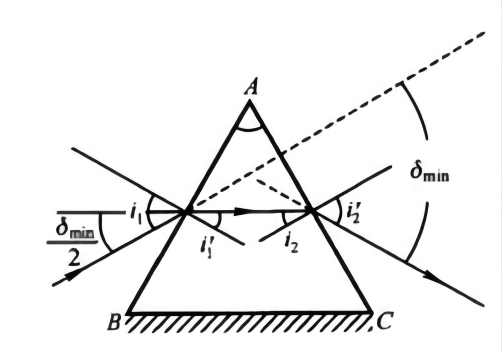
\includegraphics[width=\linewidth]{img/1.png}
        % \caption{示意图}
    \end{Figure}

    一束单色光从$AB$面以$i _1$入射后,经过棱镜的两次折射,出射角为$i ^{\prime} _2$,记偏转角为$\delta$,在顶角$\angle A$保持一定时,显然$\delta$随入射角$i _1$而改变,并且$\delta$存在最小值,对应的$i_1^{\prime} = A/2$。

    由几何关系,可以得到$i_1 = \frac 1 2 (\delta_{\min} + A)$,由此折射率$n = \dfrac{\sin i_i}{\sin A/2} = \dfrac{\sin (\delta + 1)/2}{\sin A/2}$

    \smallskip
    由此可以,通过测量顶角$\angle A$和最小偏向角$\delta_{\min}$,便可以计算棱镜的折射率$n$

    \section{实验方法}

    \subsection{调整望远镜}
    \begin{itemize}
        \item  调整望远镜目镜:调整目镜调焦手轮,使目镜中观察到的分划板刻线清晰
        \item  平行光对焦:将平面镜放在载物台上,粗调望远镜水平、载物台与望远镜垂直。在目镜中找寻镜面反射所成的绿十字的像,移动目镜筒直至清晰,并拧紧螺钉使其固定。
        \item  调整望远镜光轴使其垂直主轴:当镜面与望远镜光轴垂直时,绿十字的反射像应当落在上十字的中心如果存在偏移,适当通过调整载物台倾角和望远镜倾角可以使其回到中心。
    \end{itemize}

    \subsection{调整平行光管}

    取下平面镜,将狭缝对准汞灯光源,调整望远镜与平行光管对其,在目镜中观察狭缝像,移动狭缝筒,直至像清晰。

    为保证平行光管光轴与望远镜光轴共线,可以将狭缝旋转$90^{\circ}$,调整螺钉使像落在中心横线上,再将狭缝旋转回水平位置,锁紧螺钉。

    \subsection{测量棱镜顶角}

    对游标做标记,分别记为$K_1,K_2$,保持望远镜和刻度盘固定不动,转动游标盘,使棱镜$AC$垂直面向望远镜,分别记录下此时$K_1,K_2$的读数为$\theta_1, \theta_2$,再转动游标盘,使得$AB$盘垂直面向望远镜,分别记录下此时$K_1,K_2$的读数为$\theta_1^{\prime}, \theta_2^{\prime}$。对两次读数做差,即为载物台转过的角度:$\Phi = 1/2 (\mid \theta_1 - \theta_1^{\prime}\mid + \mid \theta_2 - \theta_2^{\prime}\mid)$

    \subsection{测量三棱镜的最小偏向角}
    \begin{itemize}
        \item 将平行光管对准前方光源
              \begin{Figure}
                  \centering
                  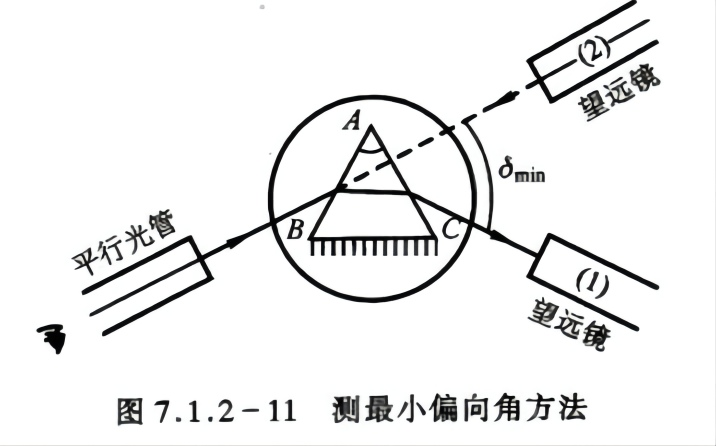
\includegraphics[width=\linewidth]{img/2.png}
                  % \caption{示意图}
              \end{Figure}
        \item 旋松望远镜止动螺钉和游标盘止动螺钉把载物台及望远镜转至如上图中所示的位置(1)处,再左右微微转动望远镜,找出棱镜出射的各种颜色的汞灯光谱线(各种波长的狭缝像)
        \item 轻轻转动载物台(改变入射角$i_1$),在望远镜中将看到谱线跟着动。改变$i_1$,应使谱线往减小的方向移动(向顶角$\angle A$方向移动)。望远镜要跟踪光谱线转动,直到棱镜继续转动,而谱线开始要反向移动(即偏向角反而变大)为止。这个反向移动的转折位置,就是光线以最小偏向角射出的方向。固定载物台,再使望远镜微动,使其分划板上的中心竖线对准其中的那条绿谱线($546.1 nm$)。
        \item 记下此时两游标处的读数$\theta_1$和$\theta_2$。取下三棱镜(载物台保持不动),转动望远镜对准平行发光管,即上图中(2)的位置,以确定入射光的方向,再记下两游标处的读数$\theta_1^{\prime}$和$\theta_2^{\prime}$。此时绿谱线的最小偏向角:

              $$
                  \delta_{\min} = 1/2 (\mid \theta_1 - \theta_1^{\prime}\mid + \mid \theta_2 - \theta_2^{\prime}\mid)
              $$
    \end{itemize}

    \section{实验数据}

    \subsection{顶角}
    \begin{tabular}{|c|c|c|c|}
        \hline \textbf{$\theta_1$}        & \textbf{$\theta_2$}       & \textbf{$\theta_1 ^{\prime}$} & \textbf{$\theta_2 ^{\prime}$} \\
        \hline  $211^{\circ} 08^{\prime}$ & $31^{\circ} 04^{\prime}$  & $92^{\circ} 08^{\prime}$      & $272^{\circ} 10^{\prime}$     \\
        \hline  $334^{\circ} 24^{\prime}$ & $154^{\circ} 23^{\prime}$ & $213^{\circ} 20^{\prime}$     & $33^{\circ} 24^{\prime}$      \\
        \hline  $95^{\circ} 37^{\prime}$  & $277^{\circ} 36^{\prime}$ & $334^{\circ} 02^{\prime}$     & $153^{\circ} 57^{\prime}$     \\\hline
    \end{tabular}

    \subsection{最小偏向角}
    \begin{tabular}{|c|c|c|c|}
        \hline \textbf{$\theta_1$}        & \textbf{$\theta_2$}       & \textbf{$\theta_1 ^{\prime}$} & \textbf{$\theta_2 ^{\prime}$} \\
        \hline  $280^{\circ} 36^{\prime}$ & $100^{\circ} 40^{\prime}$ & $219^{\circ} 00^{\prime}$     & $39^{\circ} 01^{\prime}$      \\
        \hline  $137^{\circ} 30^{\prime}$ & $317^{\circ} 30^{\prime}$ & $75^{\circ} 04^{\prime}$      & $255^{\circ} 10^{\prime}$     \\
        \hline  $86^{\circ} 31^{\prime}$  & $266^{\circ} 30^{\prime}$ & $24^{\circ} 42^{\prime}$      & $204^{\circ} 41^{\prime}$     \\\hline
    \end{tabular}

    \section{实验结果}
    \subsection{数据处理}

    测量顶角的实验中,每组的$\angle A$分别计算为:

    \begin{tabular}{|c|c|c|c|}
        \hline
                   & 1                & 2                & 3                \\\hline
        $\angle A$ & $118.95^{\circ}$ & $121.03^{\circ}$ & $122.62^{\circ}$ \\\hline
    \end{tabular}

    \smallskip
    测量偏转角的实验中,每组的$\delta_{\min}$分别计算为:

    \begin{tabular}{|c|c|c|c|}
        \hline
                        & 1               & 2               & 3               \\\hline
        $\delta_{\min}$ & $61.63^{\circ}$ & $62.38^{\circ}$ & $61.82^{\circ}$ \\\hline
    \end{tabular}

    \subsection{不确定度分析}

    注:$P=0.95$

    顶角$\angle A$的展伸不确定度:

    顶角$\angle A$的A类不确定度:

    A的样本标准差
    \begin{equation}
        \begin{aligned}
            \sigma_{\angle A} & = \sqrt{\dfrac{\Sigma_{i=1}^{n}(\angle A_i - \overline{\angle A})} {n-1}} \\
                              & = 1.83^{\circ}                                                            \\
            \mu_{\angle A}    & = \sigma_{\angle A} / \sqrt{3} = 1.06^{\circ}                             \\
        \end{aligned}
        \notag
    \end{equation}

    注意到$\theta$的测定是用类似游标卡尺的结构测定的,故置信系数取$C=\sqrt{3}$,最大允差$\Delta = 1^{\prime}$,代入公式可以得到:

    $\mu_{\angle A_{B}} = \Delta /C = 0.010 ^{\circ}$

    根据顶角的计算方法:$\pi - A = 1/2 (\mid \theta_1 - \theta_1^{\prime}\mid + \mid \theta_2 - \theta_2^{\prime}\mid)$,可以得到:$\dfrac{-\Delta A}{\pi - A} = \dfrac{\Delta \theta_1+ \Delta \theta_1^{\prime} +\Delta \theta_2+ \Delta \theta_2^{\prime}}{\mid \theta_1 - \theta_1^{\prime}\mid + \mid \theta_2 - \theta_2^{\prime}\mid}$

    因此B类不确定度为:

    $$u_B = \dfrac{\pi - A}{\mid \theta_1 - \theta_1^{\prime}\mid + \mid \theta_2 - \theta_2^{\prime}\mid} \sqrt{(4\mu_{\angle A_{B}})^2} = 0.002^{\circ}$$

    因为测量次数为3,$t_{3_{0.95}} = 4.30,k_p = 1.96$,代入公式计算$\angle A$的不确定度为:

    $U_{A0.95} = \sqrt{(t_p\mu_A)^2 + (k_p\mu_b)^2} = 0.452^{\circ}$

    用同样的办法计算$\delta_{\min}$的展伸不确定度:

    $U_{\delta_{\min}0.95} = \sqrt{(t_p\mu_A)^2 + (k_p\mu_b)^2} = 0.976^{\circ}$

    \subsection{结论}

    由$\bar n = \dfrac{\sin{\dfrac{\bar \sigma_{\min} + \bar A}{2}}}{\sin{\dfrac{\bar A}{2}}}$可以计算出,$\bar n = 1.698$

    \smallskip
    不确定度分析可以得到:

    \begin{equation}
        \begin{aligned}
            \Delta n/\bar n & = 1/2((\cot{\dfrac{\bar \delta_{\min} + \bar A}{2}-\cot{\dfrac{A}{2}}})\Delta A \\
                            & + \cot{\dfrac{\bar \delta_{\min} + \bar A}{2} \Delta \delta_{\min})             \\
        \end{aligned}
        \notag
    \end{equation}

    \smallskip
    类似的,不确定度存在如下关系:

    \begin{equation}
        \begin{aligned}
            U_n/\bar n & = 1/2((\cot{\dfrac{\bar \delta_{\min} + \bar A}{2}-\cot{\dfrac{A}{2}}})U_A \\
                       & + \cot{\dfrac{\bar \delta_{\min} + \bar A}{2} U_\delta_{\min})             \\
                       & = 0.0034
        \end{aligned}
        \notag
    \end{equation}

    因此最终测量的三棱镜折射率的结果为$n = 1.698 \pm 0.0034, P=0.95$

    标准不确定度为$0.34\%$


    \section{实验分析}


    \subsection{总结}
    虽然误差在允许范围内,但注意到实验中存在以下问题:
    \begin{itemize}
        \item 实际上不方便确定最小偏向角的位置,因为“最小值”本身难以肉眼鉴定
        \item 在观察绿光时……其宽度产生了一定的影响(难以确定中心点)
        \item 游标卡尺的读数区域有时会被支撑结构挡住,此时只能放弃这次测量,重做下一组,较为浪费时间
    \end{itemize}

    \subsection{思考题}

    已调好望远镜光轴垂直主轴,若将平面镜取下后,又放到载物台上(放的位置与拿下前的位置不同),发现两镜面又不垂直望远镜光轴了,这是为什么?是否说明望远镜光轴还没调好?

    并不。通过观察双面平面镜来调整望远镜光轴时,并未真正调平载物台,只是保证了双面镜两侧的螺钉同一高度,在平行于双面镜的方向上并未调平。
\end{multicols}
\end{document}